\pagebreak
\section{Tecnologie utilizzate}
\label{sez:tecnologie-utilizzate}

\subsection{Tecnologie di sviluppo}
\label{sez:tecnologie-sviluppo}

\subsubsection{HTML}

Linguaggio di markup standard utilizzato per creazione di pagine \textit{web}.
Permette di strutturare i contenuti di una pagina \textit{web}, andando a definire la disposizione di testo, immagini, link, tabelle, ecc.

\subsubsection{CSS}
Linguaggio di stile utilizzato per descrivere l’aspetto e la formattazione dei componenti di una pagina \textit{web}.

\subsubsection{TypeScript}

“Superset” di \textit{JavaScript}, che va ad aggiungere funzionalità e tipizzazione statica al linguaggio; 
tramite l’utilizzo di un compilatore questo viene tradotto in \textit{JavaScript} che può essere poi eseguito dai \textit{browser}.

\subsubsection{React}
Un \textit{framework} sviluppato da Meta per la creazione di interfacce \textit{web}dinamiche, permette di creare \gls{spa} tramite dei componenti riutilizzabili realizzati in file \textit{JavaScript} (.jsx) o \textit{TypeScript} (.tsx).

\subsubsection{Material UI}

Una libreria di componenti \textit{React} che implementa il \textit{Material Design}, uno stile di design sviluppato da Google.\\
Questa libreria offre un set di componenti predefiniti e pronti all’uso, che è possibile andare a personalizzare in base alle proprie esigenze.

\subsubsection{Axios}

Una libreria \textit{JavaScript} che semplifica la comunicazione tra frontend e backend, consentendo di effettuare richieste \gls{http} (GET, POST, PUT, DELETE, ecc.) in modo efficiente e personalizzabile. \\
Offre supporto per \textit{Promises}, gestione avanzata degli errori e configurazioni flessibili per adattarsi a diverse esigenze.

\subsubsection{Zod}

Una libreria \textit{TypeScript} per la validazione ed il \textit{parsing} di dati, permette di definire degli schema per strutturare e convalidare oggetti, stringhe, \textit{array}, ecc.
È possibile utilizzarla per effettuare validazioni dei dati in ingresso e in uscita dalle \gls{api}.
\subsubsection{Styled Components}

Una libreria che permette di scrivere stili CSS all’interno dei componenti \textit{React}, è possibile andare a creare stili personalizzati per ogni componente \textit{React}, andando a rendere il codice più leggibile e manutenibile.

\begin{figure}[H]
    \label{fig:styled-components}
    \centering
    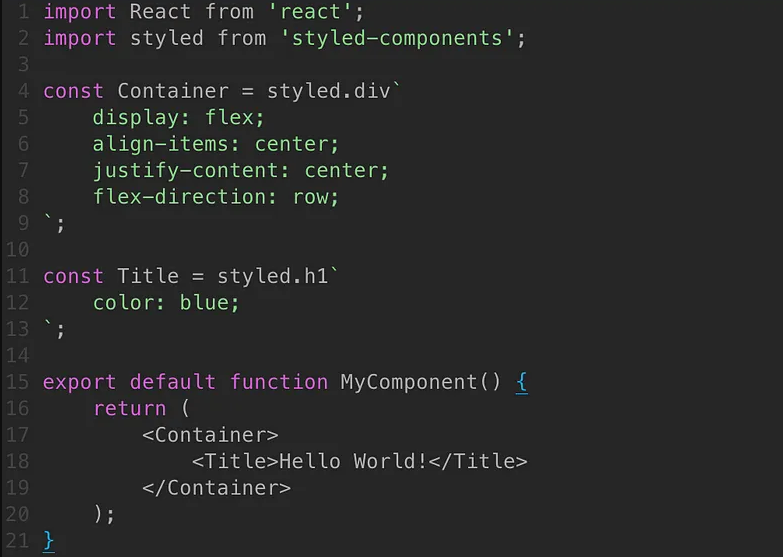
\includegraphics[scale=0.25]{tecnologie/styled-component.png}
    \caption{Esempio di utilizzo di \textit{Styled Components}}
    \cite{site:medium}
\end{figure}

\subsubsection{Vite}

Uno strumento di sviluppo utilizzato per inizializzare e configurare rapidamente il \gls{frontend} di un progetto, semplificando l'inizializzazione e ottimizzando l'esperienza di sviluppo.\\
È possibile utilizzarlo con vari \textit{framework} \gls{frontend} come ad esempio \textit{React}.

\subsubsection{React-PDF}

Libreria utilizzata per il \textit{rendering} di documenti PDF all’interno di pagine create in \textit{React}.
Consente di visualizzare, navigare ed interagire con i file PDF.

\subsubsection{Node.js}

Un ambiente di \textit{runtime JavaScript} basato sul motore V8 di \textit{Chrome}, utilizzato per eseguire codice lato \textit{server}. 
Consente di sviluppare applicazioni scalabili e ad alte prestazioni, grazie al modello asincrono e orientato agli eventi.

\subsubsection{NestJS}

Un \textit{framework} \gls{backend} moderno e robusto basato su \textit{Node.js}, progettato per creare applicazioni \textit{server} scalabili ed efficienti.
Ideale per costruire \textit{API RESTful, GraphQL} e applicazioni in tempo reale, grazie al supporto nativo per \textit{middleware}, guardie, filtri e \textit{interceptor}.
\pagebreak
\subsubsection{MongoDB}

Un \textit{database NoSQL} potente e flessibile progettato per la gestione di dati sotto forma di documenti \textit{JSON-like}. 
È ideale per applicazioni moderne grazie alla sua scalabilità orizzontale, alla capacità di gestire grandi volumi di dati non strutturati e alla facilità di integrazione con diverse tecnologie.

\begin{figure}[H]
    \label{fig:sql-nosql}
    \centering
    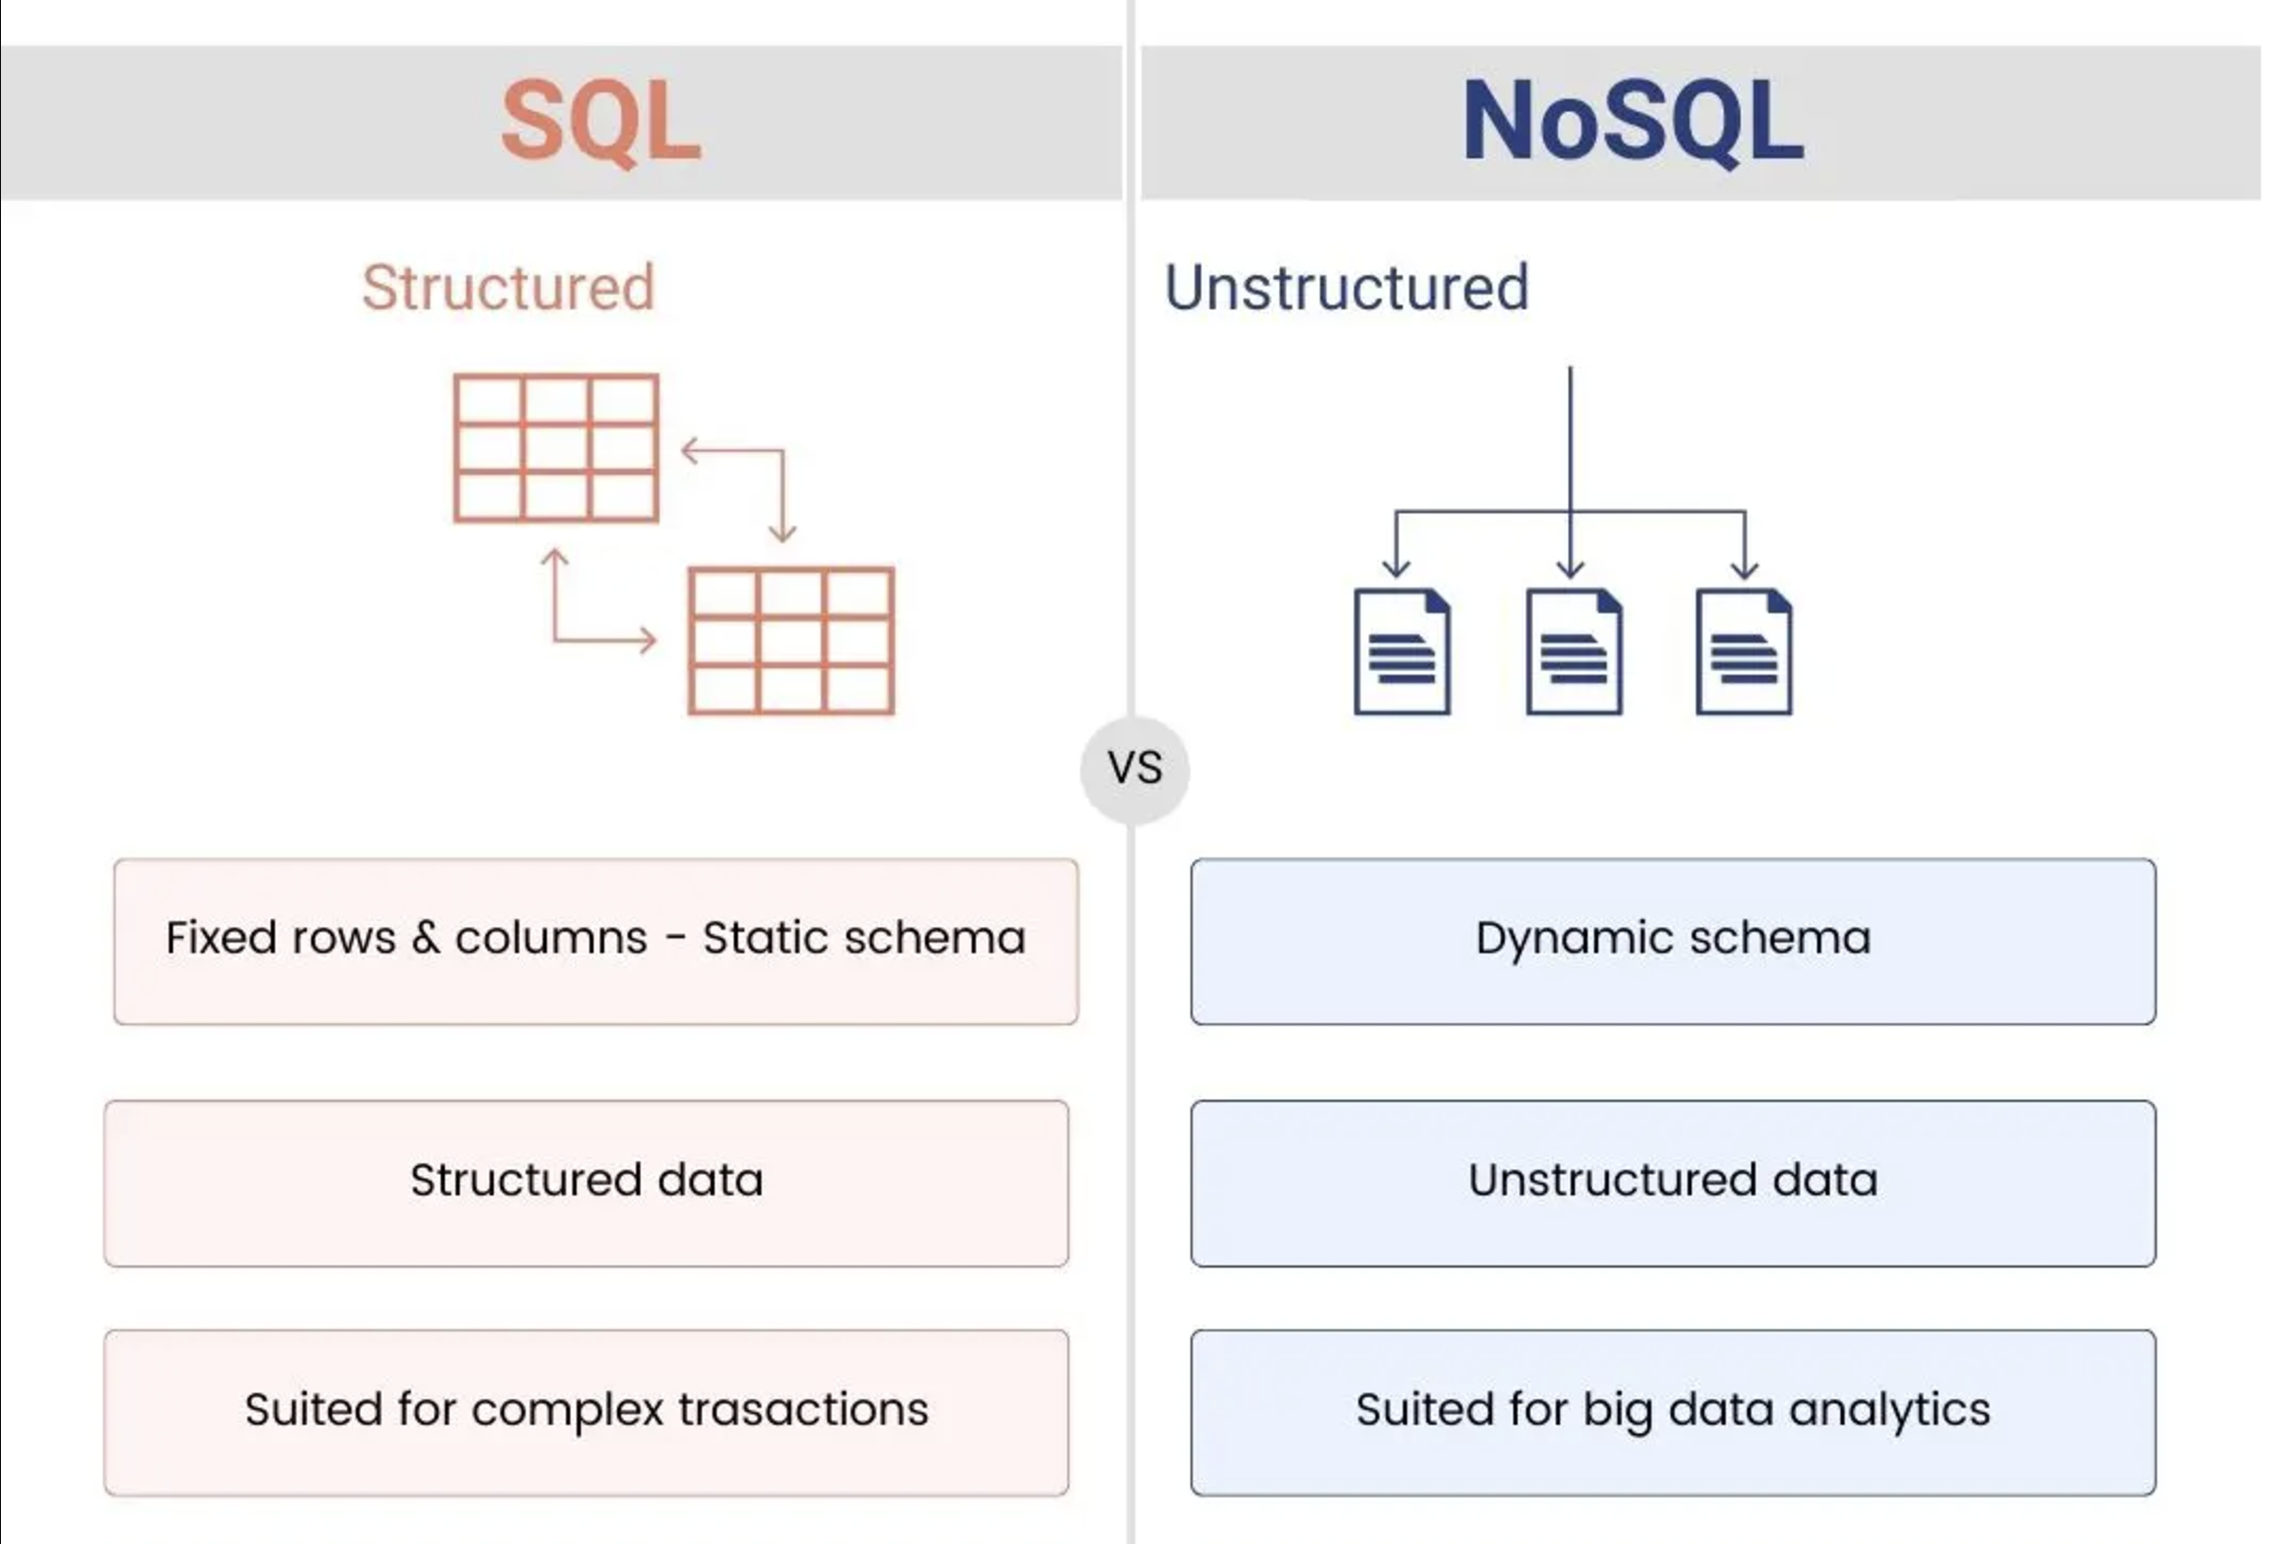
\includegraphics[scale=0.2]{tecnologie/sql-nosql.png}
    \caption{Principali differenze tra un \textit{database SQL} e un \textit{database NoSQL}}
\end{figure}

\subsubsection{Mongoose}

Un \gls{odm} per \textit{Node.js}, utilizzato per semplificare il collegamento tra \textit{NestJS} e \textit{MongoDB}. Consente di definire schemi per i dati, applicare validazioni, \textit{middleware} e trasformazioni direttamente a livello di modello. \\
\textit{Mongoose} offre un'API intuitiva per interagire con \textit{MongoDB}, supportando operazioni complesse come popolamenti, \textit{query} avanzate e gestione delle relazioni tra documenti. 

\subsubsection{LangChain}

Un \textit{framework} avanzato per lo sviluppo di applicazioni che utilizzano \gls{llm}. 
\textit{LangChain} semplifica la gestione delle chiamate \gls{api} ai modelli di linguaggio, offrendo strumenti per orchestrare flussi complessi, integrare memoria e combinare più modelli o fonti di dati.

\begin{figure}[H]
    \label{fig:langchain-usecases}
    \centering
    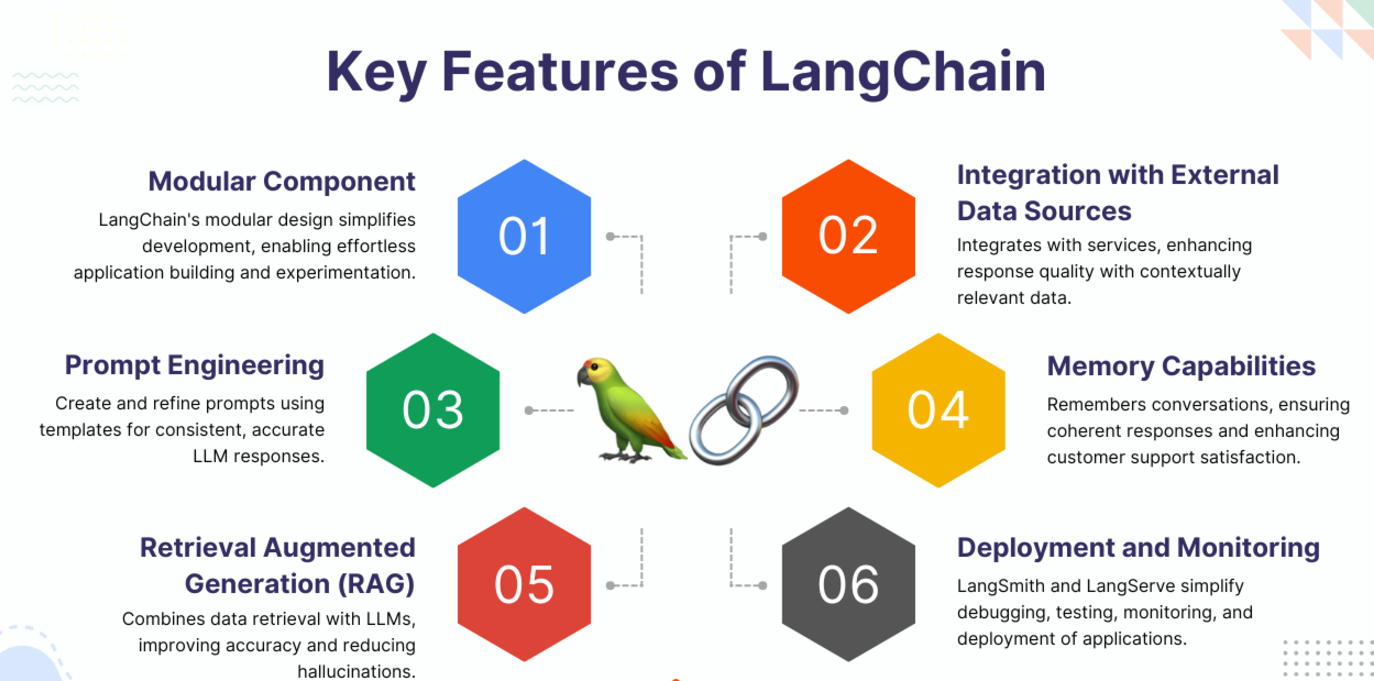
\includegraphics[scale=0.2]{tecnologie/langchain.png}
    \caption{Pricipali funzionalità di \textit{LangChain}}
\end{figure}
\subsubsection{Puppeteer}

\textit{Puppeteer} è una libreria \textit{Node.js} che controlla un \textit{browser Chromium} in modalita \textit{headless} per generare PDF da pagine \textit{web}.
È utile per creare documenti partendo da dei \textit{template}, mantenendo stili e \textit{layout}, e permettendo di personalizzare aspetti come margini e dimensioni della pagina.

\subsubsection{HandleBars}

\textit{Handlebars} è una libreria \textit{JavaScript} per creare e popolare template \textit{HTML} con dati dinamici. 
Consente di separare la logica di presentazione dai dati, supportando espressioni condizionali, \textit{loop} e \textit{helper} personalizzati.

\subsubsection{Servizi \gls{aws}}

\begin{itemize}
\item \textbf{AWS Amplify:} Una piattaforma completa per sviluppare applicazioni \textit{web} e \textit{mobile} con servizi \textit{cloud}. 
Fornisce strumenti per autenticazione, \gls{api}, storage e hosting, semplificando l'integrazione con servizi \gls{aws};
\item \textbf{AWS Cognito:} Un servizio di gestione delle identità che consente agli sviluppatori di aggiungere facilmente funzionalità di autenticazione, registrazione e accesso federato alle proprie applicazioni,
utilizzato inoltre per la generazione di \gls{jwt};
\item \textbf{AWS Bedrock:} Un servizio di intelligenza artificiale generativa offerto da \gls{aws} che consente agli sviluppatori di integrare modelli avanzati di \gls{ai} generativa nelle proprie applicazioni, senza necessità di competenze specifiche in \gls{machine-learning}. 
\textit{AWS Bedrock} supporta modelli pre-addestrati da fornitori \textit{leader} e offre funzionalità per creare, personalizzare e implementare soluzioni \gls{ai} scalabili, ideali per \textit{chatbot}, creazione di contenuti, analisi dei dati e altro;
\item \textbf{AWS S3 (Simple Storage Service):} Un servizio di archiviazione \textit{cloud} offerto da \gls{aws} progettato per il salvataggio di oggetti con scalabilità, disponibilità e sicurezza elevate.
Supporta la memorizzazione e il recupero di qualsiasi quantità di dati, con funzionalità avanzate come versionamento, controllo degli accessi e integrazione con altri servizi \gls{aws}. \\
Nel progetto specifico, \textit{AWS S3} viene utilizzato per archiviare file PDF generati dinamicamente, garantendo un accesso rapido e affidabile.
\end{itemize}

\pagebreak
\subsection{Tecnologie di supporto allo sviluppo}
\label{sez:tecnologie-supporto-sviluppo}

\subsubsection{\gls{npm}}

È il gestore ufficiale dei pacchetti per \textit{Node.js}, utilizzato per installare, condividere e gestire librerie e moduli \textit{JavaScript}. 
Facilita la configurazione e la gestione delle dipendenze nei progetti, rendendo lo sviluppo più efficiente.

\subsubsection{Docker}

Piattaforma che consente di creare e gestire applicazioni in \gls{container} leggeri e portatili.
I \gls{container} permettono l’isolazione delle applicazioni e delle loro dipendenze, garantendo consistenza tra ambienti di sviluppo, \textit{test} e produzione.

\subsubsection{Postman}

Strumento che permette di testare in modo semplice le \gls{api}. 
Consente di inviare richieste \gls{http} ed analizzare le risposte andando a semplificare lo sviluppo ed il \textit{debugging} delle \gls{api}.

\begin{figure}[H]
    \label{fig:postman}
    \centering
    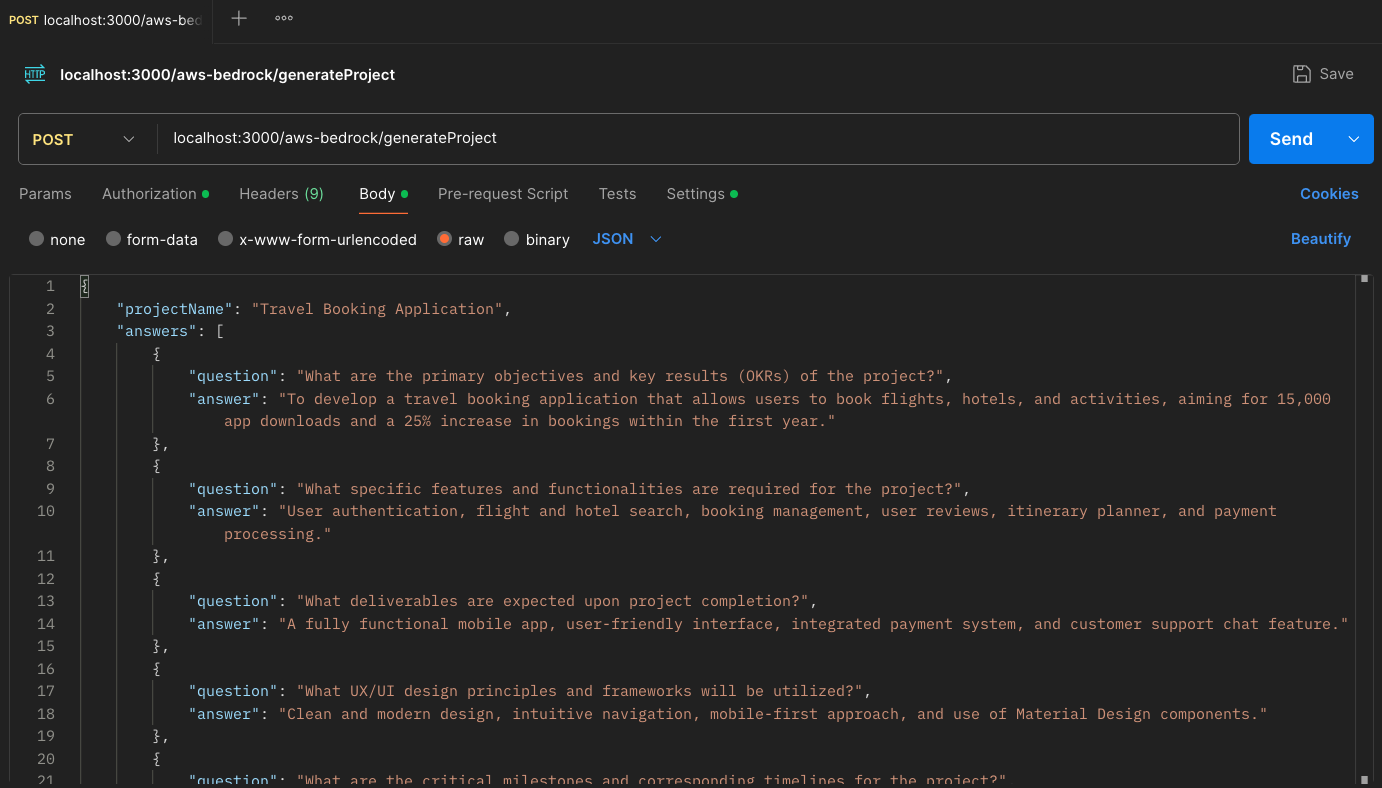
\includegraphics[scale=0.2]{tecnologie/postman.png}
    \caption{Esempio di utilizzo di \textit{Postman} per chiamata \gls{api}}
\end{figure}

\subsubsection{StarUML}

Uno strumento avanzato per la modellazione di \gls{uml}, utilizzato per creare e gestire diagrammi di progettazione software. Supporta un'ampia gamma di diagrammi \gls{uml}, tra cui casi d'uso, sequenza e attività, semplificando la visualizzazione di architetture e flussi.
È stato utilizzato per creare i diagrammi dei casi d’uso del progetto.

\subsubsection{git}

Un sistema di controllo di versione distribuito, progettato per tracciare le modifiche al codice sorgente e facilitare la collaborazione tra sviluppatori. \\
Permette di gestire versioni, ramificare progetti e integrare modifiche in modo efficiente e sicuro. 

\pagebreak
\subsubsection{MongoDB Compass}

Un'interfaccia grafica intuitiva per interagire con \textit{database MongoDB}, che consente di esplorare e modificare i dati, visualizzare indici e \textit{query},
e semplificare la gestione e l'analisi del \textit{database.}

\begin{figure}[H]
    \label{fig:mongodb-compass}
    \centering
    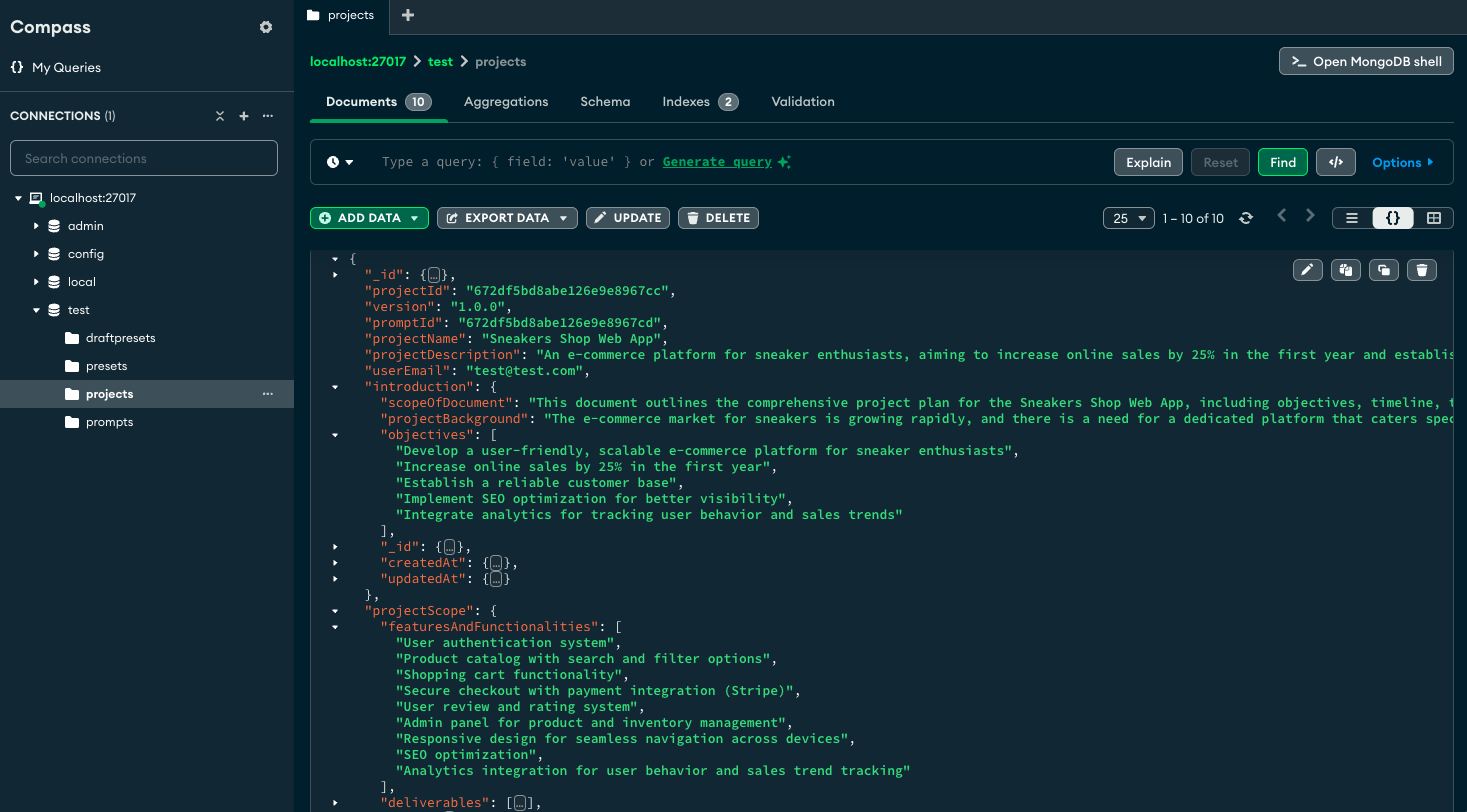
\includegraphics[scale=0.2]{tecnologie/mongodb-compass.png}
    \caption{Visualizzazione di un documento in \textit{MongoDB Compass}}
\end{figure}

\subsection{Tecnologie di verifica e validazione del codice}
\label{sez:tecnologie-validazione-codice}

\subsubsection{Jest}

\textit{Jest} è un \textit{framework} di \textit{testing JavaScript} progettato per garantire la qualità del codice, supportando \textit{test} unitari, di integrazione e \textit{snapshot}.
Grazie alla sua semplicità, velocità e funzionalità avanzate, è ideale per \textit{test} automatizzati nei progetti moderni.

\subsubsection{React Testing Library}

Una libreria per testare componenti \textit{React}, che si concentra sull'interazione dell'utente piuttosto che sull'implementazione interna. 
Fornisce strumenti per simulare eventi e verificare il comportamento dell'interfaccia utente in modo semplice e affidabile.

\subsubsection{Prettier}

Uno strumento di formattazione automatica del codice che garantisce uno stile uniforme, migliorando la leggibilità e la manutenzione del codice. 
Supporta diversi linguaggi e può essere integrato facilmente nei flussi di lavoro di sviluppo.

\subsubsection{ESLint}

Uno strumento di \textit{linting} per \textit{JavaScript} che aiuta a individuare e correggere errori nel codice, andando a migliorarne qualità e coerenza.
Supporta configurazioni personalizzabili e integrazioni con \gls{ide} per un'esperienza di sviluppo più fluida.


